
%%% main document {{{

\documentclass[
a4paper,     %% defines the paper size: a4paper (default), a5paper, letterpaper, ...
% landscape,   %% sets the orientation to landscape
% twoside,     %% changes to a two-page-layout (alternatively: oneside)
% twocolumn,   %% changes to a two-column-layout
 headsepline, %% add a horizontal line below the column title
% footsepline, %% add a horizontal line above the page footer
% titlepage,   %% only the titlepage (using titlepage-environment) appears on the first page (alternatively: notitlepage)
% parskip,     %% insert an empty line between two paragraphs (alternatively: halfparskip, ...)
% leqno,       %% equation numbers left (instead of right)
% fleqn,       %% equation left-justified (instead of centered)
% tablecaptionabove, %% captions of tables are above the tables (alternatively: tablecaptionbelow)
% draft,       %% produce only a draft version (mark lines that need manual edition and don't show graphics)
% 10pt         %% set default font size to 10 point
11pt         %% set default font size to 11 point
% 12pt         %% set default font size to 12 point
]{scrartcl}  %% article, see KOMA documentation (scrguide.dvi)



%%%%%%%%%%%%%%%%%%%%%%%%%%%%%%%%%%%%%%%%%%%%%%%%%%%%%%%%%%%%%%%%%%%%%%%%%%%%%%%%
%%%
%%% packages
%%%

%%%
%%% encoding and language set
%%%

%%% ngerman: language set to new-german
\usepackage{ngerman}

%%% babel: language set (can cause some conflicts with package ngerman)
%%%        use it only for multi-language documents or non-german ones
%\usepackage[ngerman]{babel}

%%% inputenc: coding of german special characters
\usepackage[utf8]{inputenc}

%%% fontenc, ae, aecompl: coding of characters in PDF documents
\usepackage[T1]{fontenc}
\usepackage{ae,aecompl}

%%%
%%% technical packages
%%%

%%% amsmath, amssymb, amstext: support for mathematics
%\usepackage{amsmath,amssymb,amstext}

%%% psfrag: replace PostScript fonts
\usepackage{psfrag}

%%% listings: include programming code
%\usepackage{listings}

%%% units: technical units
\usepackage{units}

%%% tiefgestellte zahlen
\usepackage{subscript}

%%% mathefoo
\usepackage{amsmath}

%%% landscape page
\usepackage{pdflscape}

\usepackage{xcolor}
% TikZ-Bibliotheken
\usepackage{tikz}
 \usetikzlibrary{backgrounds}
 \usetikzlibrary{matrix}
 \usetikzlibrary{circuits.ee.IEC}
 \usetikzlibrary{positioning}
 
 
%Hintergrundstyle - optional
\tikzstyle{background rectangle}=
  [thick,draw=\lightgray, fill=white!99!black, rounded corners]
 
%Volt- und Amperemeter festlegen:
\tikzset{circuit declare symbol = ammeter}
\tikzset{set ammeter graphic ={draw,generic circle IEC, minimum size=5mm,info=center:A}}
\tikzset{circuit declare symbol = voltmeter}
\tikzset{set voltmeter graphic ={draw,generic circle IEC, minimum size=5mm,info=center:V}}
\tikzset{circuit declare symbol = generator}
\tikzset{set generator graphic ={draw,rectangle ee, minimum size=5mm,info=center:G}}

%%%%%%%%%%%%%%%%%%%%%%%%%%%%%%%%%%%%%%%%%%%%%%%%%%%%%%%%%%%%%%%%%%%%%%%%%%
% Transistor Platzhalter, bitte durch echten Transistor ersetzen
\tikzset{circuit declare symbol = transistor}
\tikzset{set transistor graphic ={draw,generic circle IEC, minimum size=5mm,info=center:T}}
%%%%%%%%%%%%%%%%%%%%%%%%%%%%%%%%%%%%%%%%%%%%%%%%%%%%%%%%%%%%%%%%%%%%%%%%


% Spannungs und Strompfeile
\tikzset{
  Pfeil/.style={thick,shorten >=#1,shorten <=#1,->}, % für Peile
  UPfeil/.style={blue,Pfeil=#1,font={\sffamily\itshape}},% für Spannungspfeile
  IPfeil/.style={red,Pfeil=#1,font={\ttfamily\itshape}} % für Strompfeile
}


%\usepackage{circuitikz}

%Boxen
\usepackage{empheq}
 
% Command "alignedbox{}{}" for a box within an align environment
% Source: http://www.latex-community.org/forum/viewtopic.php?f=46&t=8144
\newlength\dlf  % Define a new measure, dlf
\newcommand\alignedbox[2]{
% Argument #1 = before & if there were no box (lhs)
% Argument #2 = after & if there were no box (rhs)
&  % Alignment sign of the line
{
\settowidth\dlf{$\displaystyle #1$}  
    % The width of \dlf is the width of the lhs, with a displaystyle font
\addtolength\dlf{\fboxsep+\fboxrule}  
    % Add to it the distance to the box, and the width of the line of the box
\hspace{-\dlf}  
    % Move everything dlf units to the left, so that & #1 #2 is aligned under #1 & #2
\boxed{#1 #2}
    % Put a box around lhs and rhs
}
}

%%%
%%% layout
%%%

%%% scrpage2: KOMA heading and footer
%%% Note: if you don't use this package, please remove 
%%%       \pagestyle{scrheadings} and corresponding settings
%%%       below too.
\usepackage[automark]{scrpage2}


%%%
%%% PDF
%%%

\usepackage{ifpdf}

%%% Should be LAST usepackage-call!
%%% For docu on that, see reference on package ``hyperref''
\ifpdf%   (definitions for using pdflatex instead of latex)

  %%% graphicx: support for graphics
  %\usepackage[pdftex]{graphicx}

  \pdfcompresslevel=9

  %%% hyperref (hyperlinks in PDF): for more options or more detailed
  %%%          explanations, see the documentation of the hyperref-package
  \usepackage[%
    %%% general options
    pdftex=true,      %% sets up hyperref for use with the pdftex program
    %plainpages=false, %% set it to false, if pdflatex complains: ``destination with same identifier already exists''
    %
    %%% extension options
    backref,      %% adds a backlink text to the end of each item in the bibliography
    pagebackref=false, %% if true, creates backward references as a list of page numbers in the bibliography
    colorlinks=true,   %% turn on colored links (true is better for on-screen reading, false is better for printout versions)
    %
    %%% PDF-specific display options
    bookmarks=true,          %% if true, generate PDF bookmarks (requires two passes of pdflatex)
    bookmarksopen=false,     %% if true, show all PDF bookmarks expanded
    bookmarksnumbered=false, %% if true, add the section numbers to the bookmarks
    %pdfstartpage={1},        %% determines, on which page the PDF file is opened
    pdfpagemode=None         %% None, UseOutlines (=show bookmarks), UseThumbs (show thumbnails), FullScreen
  ]{hyperref}


  %%% provide all graphics (also) in this format, so you don't have
  %%% to add the file extensions to the \includegraphics-command
  %%% and/or you don't have to distinguish between generating
  %%% dvi/ps (through latex) and pdf (through pdflatex)
  \DeclareGraphicsExtensions{.pdf}

\else %else   (definitions for using latex instead of pdflatex)

  \usepackage[dvips]{graphicx}

  \DeclareGraphicsExtensions{.eps}

  \usepackage[%
    dvips,           %% sets up hyperref for use with the dvips driver
    colorlinks=false %% better for printout version; almost every hyperref-extension is eliminated by using dvips
  ]{hyperref}

\fi


%%% sets the PDF-Information options
%%% (see fields in Acrobat Reader: ``File -> Document properties -> Summary'')
%%% Note: this method is better than as options of the hyperref-package (options are expanded correctly)
\hypersetup{
  pdftitle={}, %%
  pdfauthor={}, %%
  pdfsubject={}, %%
  pdfcreator={Accomplished with LaTeX2e and pdfLaTeX with hyperref-package.}, %% 
  pdfproducer={}, %%
  pdfkeywords={} %%
}


%%%%%%%%%%%%%%%%%%%%%%%%%%%%%%%%%%%%%%%%%%%%%%%%%%%%%%%%%%%%%%%%%%%%%%%%%%%%%%%%
%%%
%%% user defined commands
%%%

%%% \mygraphics{}{}{}
%% usage:   \mygraphics{width}{filename_without_extension}{caption}
%% example: \mygraphics{0.7\textwidth}{rolling_grandma}{This is my grandmother on inlinescates}
%% requires: package graphicx
%% provides: including centered pictures/graphics with a boldfaced caption below
%% 
\newcommand{\mygraphics}[3]{
  \begin{center}
    \includegraphics[width=#1, keepaspectratio=true]{#2} \\
    \textbf{#3}
  \end{center}
}

%%%%%%%%%%%%%%%%%%%%%%%%%%%%%%%%%%%%%%%%%%%%%%%%%%%%%%%%%%%%%%%%%%%%%%%%%%%%%%%%
%%%
%%% define the titlepage
%%%

% \subject{}   %% subject which appears above titlehead
% \titlehead{} %% special heading for the titlepage

%%% title
\title{Messbericht \\ Transistor als Schalter}

%%% author(s)
\author{Felix Schiller \\ Sebastian Littau \\ E1FS2}

%%% date
\date{Reutlingen, am 12.04.2016}

% \publishers{}

% \thanks{} %% use it instead of footnotes (only on titlepage)

% \dedication{} %% generates a dedication-page after titlepage


%%% uncomment following lines, if you want to:
%%% reuse the maketitle-entries for hyperref-setup
%\newcommand\org@maketitle{}
%\let\org@maketitle\maketitle
%\def\maketitle{%
%  \hypersetup{
%    pdftitle={\@title},
%    pdfauthor={\@author}
%    pdfsubject={\@subject}
%  }%
%  \org@maketitle
%}


%%%%%%%%%%%%%%%%%%%%%%%%%%%%%%%%%%%%%%%%%%%%%%%%%%%%%%%%%%%%%%%%%%%%%%%%%%%%%%%%
%%%
%%% set heading and footer
%%%

%%% scrheadings default: 
%%%      footer - middle: page number
\pagestyle{scrheadings}

%%% user specific
%%% usage:
%%% \position[heading/footer for the titlepage]{heading/footer for the rest of the document}

%%% heading - left
\ihead[]{Schiller, Felix \\ Littau, Sebastian}

%%% heading - center
\chead[]{Messbericht \\ Transistor als Schalter}

%%% heading - right
\ohead[]{\thepage}

%%% footer - left
% \ifoot[]{}

%%% footer - center
% \cfoot[]{}

%%% footer - right
% \ofoot[]{}



%%%%%%%%%%%%%%%%%%%%%%%%%%%%%%%%%%%%%%%%%%%%%%%%%%%%%%%%%%%%%%%%%%%%%%%%%%%%%%%%
%%%
%%% begin document
%%%

\begin{document}

% \pagenumbering{roman} %% small roman page numbers

%%% include the title
% \thispagestyle{empty}  %% no header/footer (only) on this page
\maketitle

%%% start a new page and display the table of contents
\newpage
\tableofcontents

%%% start a new page and display the list of figures
% \newpage
% \listoffigures

%%% start a new page and display the list of tables
% \newpage
% \listoftables

%%% display the main document on a new page 
% \newpage

% \pagenumbering{arabic} %% normal page numbers (include it, if roman was used above)

%%%%%%%%%%%%%%%%%%%%%%%%%%%%%%%%%%%%%%%%%%%%%%%%%%%%%%%%%%%%%%%%%%%%%%%%%%%%%%%%
%%%
%%% begin main document
%%% structure: \section \subsection \subsubsection \paragraph \subparagraph
%%%
\section{Messaufgabe}
Um das prinzipielle Schaltverhalten eines Transistors zu bestimmen, kann man diesen über den Basisstrom ansteuern und dann die Werte im \"Hauptstromkreis\" ermitteln. Dabei erkennt man die Funktionsweise des Transistors im Schaltbetrieb.

\section{Messung}
\subsection{Messschaltung}
%%%%%%%%%%%%%%%%%%%%%%%%%%%%%%%%%%%%%%%%%%%%%%%%%%%%%%%%%%%%%%%%%%%%%%%%%%%%%
% Beginn Schaltplan transistor als Schalter %%%%%%%%%%%%%%%
\begin{center}
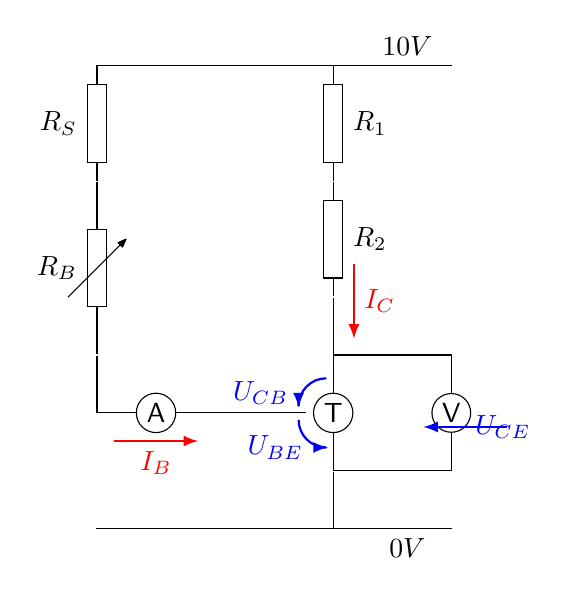
\begin{tikzpicture}[%show background rectangle,
circuit ee IEC, circuit symbol lines/.style={draw,thick},
font=\sffamily\upshape,
>=latex % Voreinstellung für Pfeilspitzen
]
\matrix (S) [
  matrix of nodes, nodes in empty cells,
  inner sep=0pt, outer sep=-.5\pgflinewidth,
  column sep=15mm, row sep = 7mm,
  nodes={minimum width=0pt}
  ]
{
  &&&  \\
  &&&  \\
  &&&  \\
  &&&  \\
  &&&  \\
  &&&  \\
  &&&  \\
  &&&  \\
  &&&  \\
};
 
 
%Orientierungshilfen
%\foreach \j in {1,...,9} %Zeilen
%{
%	\foreach \k in {1,...,4}  %Spalten
%	{%
%		\node[text=lightgray] at (S-\j-\k){+}; % Orientierungshilfe +
%		\node[red, left] at (S-\j-1){\j}; %Orientierungshilfe Zeilennummer
%		\node[red, above] at (S-1-\k){\k}; %Orientierungshilfe Spaltennummer  
%	};%
%}

%Bauteile
\draw (S-3-1) to  [resistor={info=$R_S$}](S-1-1);
\draw (S-6-1) to  [resistor={adjustable', info=$R_B$}](S-3-1);
\draw (S-7-1) to  [ammeter={name=AM1}](S-7-2);

%%%%%%%%%%%%%%%%%%%%%%%%%%%%%%%%%%%%%%%%%%%%%%
%%Transistorplatzhalter, bitte ersetzen
\draw (S-6-3) to  [transistor={name=T1}](S-8-3);
%%%%%%%%%%%%%%%%%%%%%%%%%%%%%%%%%%%%%%%%

\draw (S-6-4) to  [voltmeter={name=VM1}](S-8-4);

\draw (S-1-3) to  [resistor={info=$R_1$}, name=Wstd1](S-3-3);
\draw (S-3-3) to  [resistor={info=$R_2$}, name=Wstd2](S-5-3);

%Spannungspfeile
%Spannungspfeil der Quelle / des Voltmeters

%\draw[UPfeil=-1em]([xshift=-.5em]Gen.north west) -- node [left]{U$\mathsf{_G}$}([xshift=-.5em]Gen.south west);
\draw[UPfeil=-1em]([xshift=.5em]VM1.north east) -- node [right]{$U_{CE}$}([xshift=.5em]VM1.south east);

% U_CB
\draw[UPfeil=0em,rounded corners=10pt]
([xshift=-.25em, yshift=1.25em]T1.center) --
([xshift=-1.25em, yshift=1.25em]T1.center) --
([xshift=-1.25em, yshift=.2em]T1.center)
node[midway, left]{$U_{CB}$};

% U_BE
\draw[UPfeil=0em,rounded corners=10pt]
([xshift=-1.25em, yshift=-.25em]T1.center) --
([xshift=-1.25em, yshift=-1.25em]T1.center) --
([xshift=-.2em, yshift=-1.25em]T1.center)
node[midway, left]{$U_{BE}$};



%Strompfeile
\draw[IPfeil=-1em]([yshift=-.5em]AM1.south west) -- node [below]{$I_B$}([yshift=-.5em]AM1.south east);
\draw[IPfeil=-1em]([xshift=.75em, yshift=.2em]S-5-3.center) -- node [right]{$I_C$}([xshift=.75em, yshift=-.5em]S-5-3.center);
 
%Leiterbahnen


\draw (S-1-1) -- node[very near end, above] {$10V$}(S-1-4);
\draw (S-6-3) -- (S-6-4);
\draw (S-5-3) -- (S-6-3);
\draw (S-6-1) -- (S-7-1);
\draw (S-8-3) -- (S-8-4);
\draw (S-8-3) -- (S-9-3);
\draw (S-7-2) -- ([xshift=-1em]S-7-3.center);
\draw (S-9-1) -- node[very near end, below] {$0V$}(S-9-4);

%\draw [dashed]([xshift=-2.8em, yshift=2em]S-1-1.center) -- ([yshift=2em]S-1-2.center);
%\draw [dashed]([xshift=-2.8em, yshift=2em]S-1-1.center) -- ([xshift=-2.8em, yshift=-2em]S-3-1.center);
%\draw [dashed]([yshift=2em]S-1-2.center) -- ([yshift=-2em]S-3-2.center); 
%\draw [dashed]([xshift=-2.8em, yshift=-2em]S-3-1.center) -- ([yshift=-2em]S-3-2.center); 
 
\end{tikzpicture}
\end{center}
% Ende Schaltplan transistor als Schalter %%%%%%%%%%%%%%%
%%%%%%%%%%%%%%%%%%%%%%%%%%%%%%%%%%%%%%%%%%%%%%%%%%%%%%%%%%%%%%%%%%%%%%%%%%%%%%%%%%

\subsection{Aufbau der Schaltung}
In der oben gezeichneten Schaltung wird die Gleichstromverstärkung eines 2N3055 Transistors getestet. Als Schutzwiderstand vor der Basis des Transistors dient $R_s$ mit $10\Omega$ und $2W$ Leistung. Mit der Widerstandsdekade $R_B$ wird der Eingangsstrom in die Basis fein justiert. Der Strom $I_B$, der durch diese Strecke fließt wird mit einem Tischmultimeter von Agilent gemessen. \\
In der Collector-Emitter Strecke ist ein Lastwiderstand $R_L$ mit $11\Omega$ und $8W$ Leistung vorgeschalten. Der LAststrom wird hier mit dem Unigor A43 Analogmultimeter gemessen. Die Spannungen $U_{CB}, U_{BE}$ und $U_{CE}$ werden mit dem Fluke Multimeter gemessen.


\subsection{Messwerttabelle}
\begin{center}
\begin{tabular}{ r | r | r | r | r | r }
    $I_B$ in mA & $I_C$ in mA & $U_{CE}$ in V & $U_BE$ in V & $B$    & $P_V$ in mW \\ \hline
    0           & 0.049       & 10.01         & 0.031       & n/a    &  n/a \\
    1           & 56.2        & 9.3           & 0.683       & 56.2   & 532  \\  
    2           & 115         & 8.63          & 0.7         & 57.5   & 1009 \\
    3           & 176         & 7.9           & 0.72        & 58.6   & 1342\\
    4           & 239         & 7.17          & 0.74        & 59.75  & 1742 \\
    5           & 300         & 6.48          & 0.75        & 60     & 1976 \\
    6           & 368         & 5.77          & 0.77        & 61.3   & 2157 \\
    7           & 430         & 5.02          & 0.78        & 61.4   & 2193 \\
    8           & 490         & 4.3           & 0.8         & 61.25  & 2141 \\
    9           & 550         & 3.6           & 0.81        & 61.1   & 2012 \\
    10          & 610         & 2.9           & 0.82        & 61     & 1798 \\
    11          & 668         & 2.24          & 0.84        & 60.7   & 1520 \\
    12          & 717         & 1.67          & 0.86        & 59.7   & 1217 \\
    13          & 770         & 1.0           & 0.87        & 59.23  & 783 \\
    14          & 802         & 0.64          & 0.88        & 57.2   & 522 \\
    15          & 816         & 0.47          & 0.89        & 54.4   & 390 \\
    16          & 822         & 0.38          & 0.91        & 51.37  & 318 \\
    17          & 827         & 0.35          & 0.9         & 48.64  & 295 \\
    18          & 830         & 0.325         & 0.9         & 46.11  & 275 \\
    19          & 831         & 0.31          & 0.91        & 43.73  & 263 \\
    20          & 832         & 0.21          & 0.91        & 41.6   & 247 \\
    \hline
\end{tabular} \\
\end{center}

\subsection{Berechnung der Gleichstromverstärkung $B$ und Verlustleistung $P_V$}
Der Transistor verstärkt das Basisstrom, der über die Widerstandsdekade als Eingangssignal angelegt wird. Auf der Kollektor-Emmitter-Strecke fließt der verstärkte Strom. Diese Gleichstromverstärkung $B$ lässt sich berechnen.
\[B=\frac{I_C}{I_B}\]
Der Transistor hat einen veränderlichen Innenwiderstand. An diesem fällt ein Teil der Spannung ab und wird in Wärme umgewandelt diese Verlusleistung berechnet sich zu
\[P_V=U_{CE}\cdot(I_C+I_B)\]

\subsection{Übersteuerungsgrenze}
Die Übersteuerungsgrenze des Transistors ist erreicht, wenn die Spannung $U_{CB}$ auf $0$ abfällt. In der oben aufgebauten schaltung ist das bei den folgenden Werten der Fall:
\begin{align}
U_{BE} &= 0.89 V \nonumber \\
U_{CE} &= 0.83 V \nonumber \\
I_B    &= 13,95 mA \nonumber \\
I_C    &= 785 mA \nonumber \\
P_V    &= 663.12 mW \nonumber
\end{align}

\subsection{Zweifache Sättigung}
Im nächsten Schritt wird der Basisstrom $I_B$ verdoppelt. Die folgenden Werte können gemessen werden:
\begin{align}
U_{BE} &= 0.926 V \nonumber \\
U_{CE} &= 0.25 V \nonumber \\
I_B    &= 27.6 mA \nonumber \\
I_C    &= 835 mA \nonumber \\
P_V    &= 215.65 mW \nonumber
\end{align}
Mit steigender Übersteuerung sinkt die die Kollektor-Emitter-Spannung und damit auch der Durchlasswiderstand und die Verlustleistung. Der Transistor wird zum fast spannungsfreien Leiter. Obwohl der Durchlasswiderstand mit steigender Übersteuerung kleiner wird, ist die Übersteuerung nicht immer anzustreben, weil sie die Ausschaltzeit des Transistors stark erhöht.

\subsection{Ruhestrom im Transistor}
Um den Ruhestrom durch den Transistor messen zu können wird die Verbindung zwischen $R_B$ und der Basis gekappt. In unserem Aufbau lag er bei $I_C=49nA$.

\subsection{Durchlass- und Sperrwiderstand}
Aus den Messwerten von 2.6 und 2.7 kann der Durchlasswiderstand $R_D$ und der Sperrwiderstand $R_S$ der Kollektor Emitter-Strecke errechnet werden.
\[R_D=\frac{U_{CE}}{I_C+I_B}=\frac{0.926V}{835mA+27.6mA}=1.07\Omega\]
\[R_S=\frac{U_{CE}}{I_C+I_B}=\frac{10V}{49nA}=204M\Omega\]

\section{Auswertung und Erkenntnisse}
\subsection{Grafische Darstellung der Messwerte}
Der bei jedem eingestellten Basisstrom gemessene Kollektorstrom lässt sich in einem Diagramm darstellen. Gut zu erkennen ist der Sättigungsbereich des Transistors oberhalb von ca. $13mA$ Basisstrom.
\begin{figure}[hbtp]
\centering
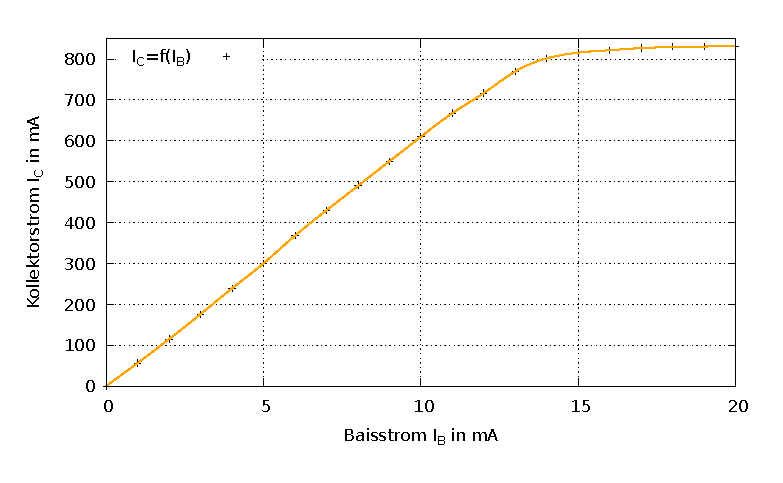
\includegraphics{kennlinie.eps}
\end{figure}

\subsection{Warum erreicht die Kennlinie die X-Achse nicht?}
Es ist im Diagramm zwar schwer zu erkennen, aber der erste Punkt im Diagramm liegt nicht auf der X-Achse. Er entspricht dem Kollektorstrom von bei uns gemessenen $49nA$ bei nicht verbundener Basis.

\subsection{An welchem Punkt der Arbeitsgeraden tritt die größte Verlustleistung auf?}
Mit Blick in die Messwerttabelle stellt man fest, dass die größte Verlustleistung in der mitte der Arbeitsgeraden, bei ca $7mA$, auftritt.

\section{Anwendungen}
\subsection{Schaltverstärker}
Eine Glühlampe für 12V mit 1W Leistung soll über einen Transistor geschaltet werden. Zur Ansteuerung der Basis wird ein Taster verwendet. 

\subsubsection*{Schaltung}
\textbf{Platzhalter Schaltplan} \\
Es gibt zwei Möglichkeiten die Schaltung aufzubauen: als Verstärkerschaltung oder in der Sättigung. Je nach Variante ist ein anderer Basiswiderstand $R_B$ notwendig.
\subsubsection*{Verstärkung}
Zum optimalen Betrieb der Lampe ist $I_C=0.166A$ notwendig. Bei einer angenommenen Gleichstromverstärkung von $B=58$ ist folgender Basisstrom notwendig:
\[I_B=\frac{I_C}{B}=\frac{0.166A}{58}=2.86mA\]
Der Basiswiderstand $R_B$ muss nun passend dimensioniert werden.
\begin{align}
R_B &= \frac{U_{RB}}{I_B} \nonumber \\
	&= \frac{12V-U_{BE}}{2.86mA} \nonumber \\
	&= \frac{12V-0.74V}{2.86mA} \nonumber \\
	&= 3937\Omega \Rightarrow R_B = 4.7k\Omega \nonumber 
\end{align}
\subsubsection*{Sättigung}
Alternativ kann der Transistor in zweifacher Sättigung betrieben werden. Die Basis-Emitter-Spannung bei zweifacher Sättigung wurde vorher zu $U_{BE}=0.72V$ gemessen, der Basisstrom zu $I_B=27.6mA$. Damit lässt sich der Basiswiderstand $R_B$ anpassen.
\begin{align}
R_B &= \frac{U_{RB}}{I_B} \nonumber \\
	&= \frac{12V-0.72V}{27.6mA} \nonumber \\
	&= 408\Omega \Rightarrow R_B = 470\Omega \nonumber 
\end{align}
In beiden Varianten kommt man zu identischen Ergebnissen. die an der Lampe $H_1$ gemessene Spannung beträgt beides mal $U_{H_1}\approx 11.7V$.

\subsection{Bistabile Kippstufe}
\subsubsection*{Schaltplan}
\textbf{Platzhalter Schaltplan} \\
Folgende Bauteile wurden in der Schaltung verwendet:
\[T_1=T_2=BC140, R_2=R_3=1k\Omega, R_1=R_4=470\Omega, U_B=7V\]
\subsubsection*{Aufbau der Schaltung}
In dem Moment in dem eine Versorgungsspannung an die Schaltung gelegt wird, gibt es noch keinen definierten Zustand. Es ist dem Zufall überlassen, ob $T_1$ oder $T_2$ zuerst durchschaltet. Angenommen, $T_1$ würde zuerst durchschalten, dann würde zunächst einmal die LED $L_2$ leuchten. An ihr liegt die nötige Spannung an, da $T_2$ sperrt. Dafür wird der Basisanschluss von $T_2$ auf Massepotential gebracht, da er über $R_2$ mit dem Kollektor des durchgeschaltenen $T_1$ verbunden ist und damit quasi auf Masse liegt. Die LED $L_1$ leuchtet nicht, da beide Anschlüsse auf dem selben Potential liegen. Wird nun der Schalter $S_1$ gedrückt, liegt die Basis von $T_1$ auf Massepotential. $T_1$ sperrt, $L_1$ leuchtet auf, und die Basis von $T_2$ kann über $R_2$ mit Strom versorgt werden, $T_2$ schaltet. Auch beim Loslassen von $S_1$ bleibt dieser Zustand erhalten, da nun die Basis von $T_1$ durch $T_2$ auf Masssepotential gebracht wird.
Der gleiche Vorgang ist natürlich auch umgekehrt mit dem Schalter $S_2$ möglich. Dieser kann die LED $L_2$ einschalten und $L_1$ ausschalten.

\subsection{Astabiler Multivibrator}
\subsubsection{Schaltung}
\textbf{Platzhalter Schaltplan} \\
Folgende Bauteile wueden in der Schaltung verwendet: 
\[T_1=T_2=BC140, R_1=R_2=1k\Omega, R_2=R_3=15k\Omega, C_1=C_2=47\mu F, U_B=7V\]
\subsubsection{Aufbau der Schaltung}
Der astabile Multivibrator ist fast identisch zur bistabilen Kippstufe. Die Schalter werden nun aber durch RC-Glieder ersetzt.

\subsubsection{Funktionsweise der astabilen Kippstufe}
Da es keinen definierten Ausgangszustand gibt, wird zunächst davon ausgegangen, dass der Transistor $T_1$ gerade durchschaltet.
Wenn der Transistor $T_1$ durchschaltet, dann erlischt zunächst einmal die LED $L_1$. Gleichzeitig wird der Transistor $C_1$ auf der $T_1$ zugewandten Seite auf Masse gezogen. Dieser negative Spannungssprung (von 7V, wenn $T_1$ sperrt auf 0V wenn $T_1$ leitet) wird über den Kondensator $C_1$ (der Spannungssprung ist wie eine kurzzeitige Wechselspannung, kann also den Kondensator durchdringen) auf die Basis von $T_2$ übertragen, welcher somit sperrt. Die LED $L_2$ leuchtet also. Während nun der $T_1$ leitet, wird $C_1$ über $R_2$ langsam aufgeladen und sobald der Kondensator eine Spannung von 0,7V erreicht hat, schaltet $T_2$ durch. Die LED $L_2$ erlischt und gleichzeitig wird $C_2$ am Anschluss bei $T_2$ auf 0V gezogen und überträgt dadurch wiederrum einen negativen Spannungssprung auf die Basis von $T_1$. Dieser sperrt, $L_1$ leuchtet auf. Nun wird $C_2$ über $R_3$ langsam aufgeladen und beim Erreichen von 0,7V leitet $T_1$ wieder, der Kreislauf beginnt von vorne.
\subsubsection{Veränderungen der Kapazitäten und Widerstände}
\begin{itemize}
\item Bei Verdoppelung der Kapazitäten $C_1$ und $C_2$ blinken die LEDs mit deutlich niedrigerer Frequenz. Die größeren Kondensatoren brauchen eine längere Zeit, bis sie auf die Schaltspannung der Transistoren aufgeladen sind.
\item Bei Halbierung der Widerstandswerte $R_2$ und $R_3$ blinken die LEDs in deutlich höherer Frequenz. Durch die niederohmigeren Widerstände fließt ein höherer Aufladestrom in die Kondensatoren. Die Transistoren schalten nach kürzerer Zeit durch.
\item Bei asymmetrischer Änderung der Widerstandswerte und Kapazitäten ändert sich auch die Frequenz hin zm asymmetrischen. Halbiert man z.B. nur $R_1$ und $C_2$, belässt aber $R_3$ und $C_1$ auf den ursprünglichen Werten, so blinkt $L_2$ immer nur kurz auf, während $L_1$ unverändert lange leuchtet.
\end{itemize}

%%%
%%% end main document
%%%
%%%%%%%%%%%%%%%%%%%%%%%%%%%%%%%%%%%%%%%%%%%%%%%%%%%%%%%%%%%%%%%%%%%%%%%%%%%%%%%%

% \appendix  %% include it, if something (bibliography, index, ...) follows below

%%%%%%%%%%%%%%%%%%%%%%%%%%%%%%%%%%%%%%%%%%%%%%%%%%%%%%%%%%%%%%%%%%%%%%%%%%%%%%%%
%%%
%%% bibliography
%%%
%%% available styles: abbrv, acm, alpha, apalike, ieeetr, plain, siam, unsrt
%%%
% \bibliographystyle{plain}

%%% name of the bibliography file without .bib
%%% e.g.: literatur.bib -> \bibliography{literatur}
% \bibliography{FIXXME}

\end{document}
%%% }}}
%%% END OF FILE
%%%%%%%%%%%%%%%%%%%%%%%%%%%%%%%%%%%%%%%%%%%%%%%%%%%%%%%%%%%%%%%%%%%%%%%%%%%%%%%%
%%% Notice!
%%% This file uses the outline-mode of emacs and the foldmethod of Vim.
%%% Press 'zi' to unfold the file in Vim.
%%% See ':help folding' for more information.
%%%%%%%%%%%%%%%%%%%%%%%%%%%%%%%%%%%%%%%%%%%%%%%%%%%%%%%%%%%%%%%%%%%%%%%%%%%%%%%%
%% Local Variables:
%% mode: outline-minor
%% OPToutline-regexp: "%% .*"
%% OPTeval: (hide-body)
%% emerge-set-combine-versions-template: "%a\n%b\n"
%% End:
%% vim:foldmethod=marker
